%   % !TEX root = ../../VIII,3_Rahmen-TeX_8-1.tex
%
%
%   Band VIII, 3 N.~??A45
%   Signatur/Tex-Datei: LH_37_05_180
%   RK-Nr. 60353
%   \ref{RK60353}
%   Überschrift: Restitutio isochrona elastri
%   Modul: AEF / Elastizität
%   Datierung: ??? 1690 bis 1695 ???
%   WZ:
%.      LEd-WZ 803042 = RK-WZ 455, 514, 7e (insgesamt: eins)
%   SZ:   (?????)
%   Bilddateien (PDF):
%      LH_37_05_180_d1  ((ex: lh037_05_180r-d1))
%      LH_37_05_180_d2  ((ex: lh037_05_180r-d2))
%      LH_37_05_180_d3  ((ex: lh03705_180v-d1))
%      LH_37_05_180_d4  ((ex: lh03705_180v-d2))
%      LH_37_05_180_d5  ((ex: lh03705_180v-d3))
%      (insgesamt: fünf)
%   Verzeichniseinträge: vollständig
%   \textls{} statt \textso{} (Ausnahme: Personenverzeichnis)
%
%
\selectlanguage{ngerman}%
\frenchspacing%
%
\begin{ledgroupsized}[r]{120mm}%
\footnotesize%
\pstart%
\noindent\textbf{Überlieferung:}%
\pend%
\end{ledgroupsized}%
\begin{ledgroupsized}[r]{114mm}%
\footnotesize%
\pstart%
\parindent -6mm%
\makebox[6mm][l]{\textit{L}}%
Konzept:
LH~XXXVII~5 Bl.~180.
Ein Blatt 2\textsuperscript{o};
ein Wasserzeichen; Papiererhaltungsmaßnahmen.
Zwei vollbeschriebene Seiten.
Die Randbemerkungen wurden zumeist nach der Anfertigung von N.~\ref{RK60301} hinzugefügt.%
\pend%
\end{ledgroupsized}%
%
%\vspace*{5mm}
%\begin{ledgroup}
%\footnotesize
%\pstart
%\noindent
%\textbf{Datierungsgründe}: Noch nicht datiert. WZ.
%\pend
%\end{ledgroup}
%
\selectlanguage{latin}%
\frenchspacing%
%
%
\vspace{8mm}%
\normalsize%
 \count\Bfootins=1100
\count\Afootins=1200
\count\Cfootins=1100
\pstart%
\noindent%
%
\lbrack180~r\textsuperscript{o}\rbrack%    %%%%    Blatt 180r
%
\hspace{27mm}%
\textls{Restitutio Isochrona Elastri,}%
\protect\index{Sachverzeichnis}{restitutio isochrona}%
\protect\index{Sachverzeichnis}{restitutio elastri}%
\protect\index{Sachverzeichnis}{elastrum}%
\protect\index{Sachverzeichnis}{isochronismus restitutionis}
%
\edlabel{LH_37_05_180_m180r1}%
etc.%
\edtext{}{%
{\xxref{LH_37_05_180_m180r1}{LH_37_05_180_m180r2}}%
{\lemma{etc.}\Bfootnote{%
\textit{(1)}~Si
\textit{(2)}~Motus ad
\textit{(a)}~scopum
\textit{(b)}~terminum%
~\textit{L}}}}%
%
\edlabel{LH_37_05_180r_inaliaplagula-1}%
\edtext{}{%
\lemma{\textit{Am oberen Rand:}}\Afootnote{%\hspace{1,6mm}\killnumber
Ubi lapsus indicat NB NB%
\protect\index{Sachverzeichnis}{lapsus}%
\textsuperscript{\lbrack a\rbrack}
in hac et sequente pagina,%
\protect\index{Sachverzeichnis}{pagina}
Rem praeclare absolvi in alia plagula.%
\protect\index{Sachverzeichnis}{plagula}%
\textsuperscript{\lbrack b\rbrack}%
{\footnotesize%
\newline\vspace{-0.5em}%
\newline%
\textsuperscript{\lbrack a\rbrack}~NB NB \lbrack...\rbrack\ pagina:
Vgl. die Randbemerkungen auf
S.~\refpassage{LH_37_05_180_rndbmerk_1-1}{LH_37_05_180_rndbmerk_1-2};
\refpassage{LH_37_05_180_rndbmerk_2-1}{LH_37_05_180_rndbmerk_2-2};
\refpassage{LH_37_05_180_rndbmerk_3-1}{LH_37_05_180_rndbmerk_3-2};
\refpassage{LH_37_05_180_rndbmerk_4-1}{LH_37_05_180_rndbmerk_4-2}.
%
\quad%
\textsuperscript{\lbrack b\rbrack}~in alia plagula:
Siehe N.~\ref{RK60301}.%, S.~\refpassage{}{}.???%
\newline%
}}}%
\edlabel{LH_37_05_180r_inaliaplagula-2}%
%
\edtext{}{%
\lemma{\textit{Über dem Titel:}}\Afootnote{%\hspace{1,6mm}\killnumber
Hic quaedam sub finem%
\textsuperscript{\lbrack a\rbrack}
notanda de relationibus generalibus in calculo.%
\protect\index{Sachverzeichnis}{relatio generalis in calculo}%
{\footnotesize%
\newline\vspace{-0.5em}%
\newline%
\textsuperscript{\lbrack a\rbrack}~sub finem:
Vgl. die Randbemerkung auf 
S.~\refpassage{LH_37_05_180_rndbmerk_5-1}{LH_37_05_180_rndbmerk_5-2}.%S.~\pageref{LH_37_05_180v_marg_srh}.%
}}}%
\pend%
\vspace{0.5em}%
%
\pstart%
\noindent%
Motus%
\edlabel{LH_37_05_180r_Anfang-1}
ad terminum%
\edlabel{LH_37_05_180_m180r2}
ea
%
\edtext{lege tendit,%
\protect\index{Sachverzeichnis}{motus ad terminum tendens}%
\protect\index{Sachverzeichnis}{lex motus ad terminum}%
}{%
\lemma{lege}\Bfootnote{%
\textit{(1)}~tendat
\textit{(2)}~si tendat
\textit{(3)}~tendit,%
~\textit{L}}}
%
ut quantum virium%
\protect\index{Sachverzeichnis}{vis recepta a mobile}
%
\edtext{mobile ad eum tendendo recepit,
de vi causae}{%
\lemma{mobile}\Bfootnote{%
\textit{(1)}~tendenda rece
\textit{(2)}~ad eum tendendo recepit,
\textit{(a)}~causa
\textit{(b)}~termin
\textit{(c)}~de vi causae%
~\textit{L}}}
%
agendi decedat,%
\protect\index{Sachverzeichnis}{vis causae agendi}
%
\edtext{solicitatioque%
\protect\index{Sachverzeichnis}{solicitatio pergendi}
ipsa pergendi hinc diminuatur,}{%
\lemma{solicitatioque}\Bfootnote{%
\hspace{-0,5mm}ipsa pergendi hinc diminuatur,
\textit{erg.~L}}}
%
si scilicet unum idemque semper sit agens,%
\protect\index{Sachverzeichnis}{agens unum idemque}
neque aliud quam hoc agat.%
\edlabel{LH_37_05_180r_Anfang-2}
Sed tale quid non fit in gravitate.%
\protect\index{Sachverzeichnis}{gravitas}
%
\edtext{Nam solicitatio gravis%
\protect\index{Sachverzeichnis}{solicitatio gravis}
ad descendendum non%
\protect\index{Sachverzeichnis}{solicitatio ad descendendum}%
}{%
\lemma{Nam}\Bfootnote{%
\textit{(1)}~non
\textit{(2)}~solicitatio gravis ad descendendum non%
~\textit{L}}}
%
ideo minuitur,
quod diu jam descendit.
Et licet toti aetheri%
\protect\index{Sachverzeichnis}{aether}
tantum virium decesserit,%
\protect\index{Sachverzeichnis}{vis aetheri decessa}
quantum gravi accessit;%
\protect\index{Sachverzeichnis}{vis gravi accessa}
sequitur hinc quidem
omnia gravia totius
%
\edtext{orbis,%
\protect\index{Sachverzeichnis}{orbis}
vel quaecunque vi aetheris urgentur,%
\protect\index{Sachverzeichnis}{vis aetheris}
tanto minus}{%
\lemma{orbis,}\Bfootnote{%
\textit{(1)}~tanto mi
\textit{(2)}~vel quaecunque \lbrack...\rbrack\ tanto minus%
~\textit{L}}}
%
urgeri,
sed non in hoc praesens grave urgendum%
\protect\index{Sachverzeichnis}{grave urgendum}
refundi hoc detrimentum.%
\protect\index{Sachverzeichnis}{detrimentum}
Neque sane eae partes aetheris%
\protect\index{Sachverzeichnis}{aether}%
\protect\index{Sachverzeichnis}{pars aetheris}
quae vim amisere%
\protect\index{Sachverzeichnis}{vis aetheris amissa}%
\lbrack,\rbrack\
grave
in quo amisere
inter descendendum comitantur,
sed aliae%
\protect\index{Sachverzeichnis}{pars aetheris}
viribus integris%
\protect\index{Sachverzeichnis}{vis integra}
in ipsum agunt.
%
\edtext{Videndum an in vi elastica%
\protect\index{Sachverzeichnis}{vis elastica}
\lbrack habeatur\rbrack\
totum quod posuimus.
Atque ita certa moderatione videtur.}{%
\lemma{Videndum}\Bfootnote{%
\hspace{-0,5mm}an in vi elastica
\textbar~habeat \textit{ändert Hrsg.}~%
\textbar\ totum quod posuimus.
\textit{(1)}~Atque ita sane videtur
\textit{(2)}~Atque ita certa moderatione videtur.
\textit{erg.~L}}}%
\pend%
% \newpage%
%
\pstart%
Si motus ad terminum%
\protect\index{Sachverzeichnis}{motus ad terminum tendens}
ea lege tendat,%
\protect\index{Sachverzeichnis}{lex motus ad terminum}
%
\edtext{ut quanto}{%
\lemma{ut}\Bfootnote{%
\textit{(1)}~quantum
\textit{(2)}~quanto%
~\textit{L}}}
%
minus ab eo abest,
tanto minus urgeatur,
videndum
quae inde consequantur.
Abesse autem,
seu distantia,%
\protect\index{Sachverzeichnis}{distantia a termino}
hic non semper sumitur in loco,
sed et in gradu diversitatis,%
\protect\index{Sachverzeichnis}{gradus diversitatis}%
\protect\index{Sachverzeichnis}{distantia sumta in gradu diversitatis}
ut in tensione.%
\protect\index{Sachverzeichnis}{gradus tensionis}%
\protect\index{Sachverzeichnis}{tensio}
Sed tunc variis rursus modis sumi potest,
et cogitandum est de mensura homogenea certa%
\protect\index{Sachverzeichnis}{mensura homogenea}%
\lbrack:\rbrack\
ut in Elastri tensione,%
\protect\index{Sachverzeichnis}{tensio elastri}%
\protect\index{Sachverzeichnis}{elastrum}
si
cum aer comprimitur,%
\protect\index{Sachverzeichnis}{aer compressus}
intelligatur vis Elastica%
\protect\index{Sachverzeichnis}{vis elastica}
esse ut densitates%
\protect\index{Sachverzeichnis}{densitas}
seu ut spatia.%
\protect\index{Sachverzeichnis}{spatium}
An dicemus vim%
\protect\index{Sachverzeichnis}{vis elastica}
%
\edtext{elasticam dependere ab exiguitate}{%
\lemma{elasticam}\Bfootnote{%
\textit{(1)}~esse proportionatam exigu
\textit{(2)}~dependere ab exiguitate%
~\textit{L}}}
%
intervallorum%
\protect\index{Sachverzeichnis}{intervallum per quod aether transit}%
\protect\index{Sachverzeichnis}{exiguitas intervallorum}%
\protect\index{Sachverzeichnis}{transitus aetheris}
per quae transit aether,%
\protect\index{Sachverzeichnis}{aether}
quod ille transire debeat
eadem qua ante celeritate%
\lbrack?\rbrack\
Sed hoc dicere non licet,
quia
cum desinitur in infinite parva intervalla,%
\protect\index{Sachverzeichnis}{intervallum infinite parvum}
fieret tunc transitus infinite velox%
\protect\index{Sachverzeichnis}{transitus infinite velox}
seu vi summa,%
\protect\index{Sachverzeichnis}{vis summa}
cum tamen revera sit
%
\edlabel{LH_37_05_180_m180r3}%
nulla.%
\protect\index{Sachverzeichnis}{vis nulla}%
%
\edtext{}{%
{\xxref{LH_37_05_180_m180r3}{LH_37_05_180_m180r4}}%
{\lemma{nulla.}\Bfootnote{\hspace{-0,5mm}%
\lbrack/\rbrack\
\textit{(1)}~Sit
\textit{(2)}~Videa
\textit{(3)}~Illud%
~\textit{L}}}}%
\pend%
\pstart%
Illud%
\edlabel{LH_37_05_180_m180r4}
%
in Elastris omnibus nobis obviis,%
\protect\index{Sachverzeichnis}{elastrum soni capax}
%
\edtext{soni%
\protect\index{Sachverzeichnis}{sonus} capacibus}{%
\lemma{soni}\Bfootnote{\hspace{-0,5mm}%
\textbar~nempe \textit{gestr.}~%
\textbar\ capacibus%
~\textit{L}}}
%
deprehendimus,
ut
%
\edtext{restitutiones sint aequiveloces,%
\protect\index{Sachverzeichnis}{restitutio aequivelox}
sive plus sive minus a quiete%
\protect\index{Sachverzeichnis}{quies}%
\protect\index{Sachverzeichnis}{recessus a quiete}%
\protect\index{Sachverzeichnis}{recessus a termino}
seu
%
\edtext{termino recesserint.}{%
\lemma{termino}\Bfootnote{%
\textit{(1)}~descenderint.
\textit{(2)}~recesserint.%
~\textit{L}}}%
}{%
\lemma{restitutiones \lbrack...\rbrack\ recesserint}\Cfootnote{%
Es ist wohl gemeint, dass die einzelnen Schwingungen einer Saite (\textit{caeteris paribus}) eine von deren Auslenkung unabhängige, konstante Dauer aufweisen.}}
%
Videndum
%
\edtext{est,
an aliquid}{%
\lemma{est,}\Bfootnote{%
\textit{(1)}~quid hinc
\textit{(2)}~an aliquid%
~\textit{L}}}
%
inde colligi de lege solicitationis%
\protect\index{Sachverzeichnis}{lex solicitationis}
possit.
Sit
%
\edtext{tempus \textit{AT},%
\protect\index{Sachverzeichnis}{tempus restitutionis}%
}{%
\lemma{tempus \textit{AT}}\Cfootnote{%
Vgl. das Diagramm \lbrack\textit{Fig.~1}\rbrack.}}
%
solicitatio impressa \makebox[1.0\textwidth][s]{\textit{TC},%
\protect\index{Sachverzeichnis}{solicitatio impressa}
quae semper minuitur
donec evanescat%
\protect\index{Sachverzeichnis}{solicitatio evanescens}
transcurso tempore \textit{AE}.%
\protect\index{Sachverzeichnis}{tempus restitutionis}
Hanc solicitationem}
\pend
  \vspace{2.5em}%	% Diagramm Fig.~1
  \centerline{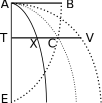
\includegraphics[width=0.24\textwidth]{gesamttex/edit_VIII,3/images/LH_37_05_180_d1.pdf}}%
  \vspace{0.5em}
  \centerline{\lbrack\textit{Fig.~1}\rbrack}%
  \label{LH_37_05_180r_Fig.1}%
 % \vspace{1.5em}%
\newpage
\pstart
\noindent intelligo accedendi ad%
\protect\index{Sachverzeichnis}{solicitatio accedendi ad terminum}
%
\edtext{terminum.
Velocitas%
\protect\index{Sachverzeichnis}{velocitas accedendi ad terminum}
%
ad terminum accedendi % ,
ponatur ex solicitationibus composita,%
\protect\index{Sachverzeichnis}{solicitatio accedendi ad terminum}%
\protect\index{Sachverzeichnis}{velocitas a solicitationibus composita}%
\protect\index{Sachverzeichnis}{terminus motus}
quae sit \textit{TV};
erit
$\displaystyle TV = 
\!\int\!\! TCdAT.$%
\textls{ Accessiones }%
\protect\index{Sachverzeichnis}{accessio ad terminum}%
}{%
\lemma{terminum.}\Bfootnote{%
\textit{(1)}~Et quae sit \textit{TV}
\textit{(2)}~Et sunt \textit{TV} ipsis \textit{AVL} pro areis \textit{BAT} proportionales \textit{TU}
\textit{(3)}~Et velocitatem
\textit{(4)}~Velocitatem
\textit{(5)}~Velocitas ad % ...
\lbrack...\rbrack\ $\displaystyle TV = \!\int\!\! TCdAT.$
\textit{(a)}~Porro
\textit{(b)}~\textls{Accessiones}%
~\textit{L}}}%
%
autem ad
%
\edtext{terminum%
\protect\index{Sachverzeichnis}{terminus motus}
sunt in ratione composita
elementorum temporis%
\protect\index{Sachverzeichnis}{elementum temporis}
et velocitatum%
\protect\index{Sachverzeichnis}{elementum velocitatis}%
\lbrack,\rbrack\
et%
\textls{ accessus }%
\protect\index{Sachverzeichnis}{accessus ad terminum}%
\edtext{\textit{TM}}{%
\lemma{\textit{TM}}\Cfootnote{%
Der Punkt \textit{M} ist im Diagramm \lbrack\textit{Fig.~1}\rbrack\ auf S.~\pageref{LH_37_05_180r_Fig.1} nicht eingezeichnet.}}
sunt summae accessionum,%
\protect\index{Sachverzeichnis}{accessio ad terminum}
adeoque $\displaystyle TM = \!\int\!\! \overline{TVdt}.$%
}{%
\lemma{terminum}\Bfootnote{%
\hspace{-0,5mm}sunt
\textit{(1)}~ut
\textit{(2)}~in
\textit{(a)}~compo
\textit{(b)}~ratione composita elementorum temporis et
\textit{(aa)}~velocitatis
\textit{(bb)}~velocitatum et \textls{accessus}
\textbar~\textit{TM} \textit{erg.}~\textbar~%
\textit{(aaa)}~seu ele
\textit{(bbb)}~seu
\textit{(ccc)}~sunt summae
\textit{(aaaa)}~ascensio
\textit{(bbbb)}~accessionum,
\textit{(aaaaa)}~sunt itaque
\textit{(bbbbb)}~accessiones si
\textit{(ccccc)}~adeoque $\displaystyle TM = \!\int\!\! \overline{TVdt}.$%
~\textit{L}}}
%
%\pend%
%%
%\pstart%
Sed brevius rem literis simplicibus%
\protect\index{Sachverzeichnis}{litera simplex}
%
\edtext{trademus,
Tempus \textit{AT} sit \textit{t},%
\protect\index{Sachverzeichnis}{tempus restitutionis}%
}{%
\lemma{trademus,}\Bfootnote{%
\textit{(1)}~sit
\textit{(2)}~Tempus \textit{AT} sit \textit{t},%
~\textit{L}}}
%
Solicitatio%
\protect\index{Sachverzeichnis}{solicitatio accedendi ad terminum}
%
\edtext{\textit{TL}}{%
\lemma{\textit{TL}}\Cfootnote{%
Der Punkt \textit{L} ist im Diagramm \lbrack\textit{Fig.~1}\rbrack\ auf S.~\pageref{LH_37_05_180r_Fig.1} nicht eingezeichnet.}}
%
sit \textit{c},
%
\edtext{Velocitas \textit{TV} sit%
\protect\index{Sachverzeichnis}{velocitas accedendi ad terminum}
$v \stackrel{(1)}{=} \displaystyle \!\int\!\! \overline{c\,dt},$
Accessio erit \textit{v\,dt},%
\protect\index{Sachverzeichnis}{accessio ad terminum}%
}{%
\lemma{Velocitas}\Bfootnote{%
\textit{(1)}~seu accessio s
\textit{(2)}~sit
\textit{(3)}~\textit{TV} sit % $v n\stackrel{(1)}{=} \displaystyle \!\int\!\! \overline{c\,dt},$ Accessio 
\lbrack...\rbrack\ erit \textit{v\,dt},%
~\textit{L}}}
%
ipse Accessus%
\protect\index{Sachverzeichnis}{accessus ad terminum}
$x \stackrel{(2)}{\text{erit}} \displaystyle \!\int\!\! \overline{v\,dt}.$
Adeoque
$x \stackrel{(3)}{=} \displaystyle \!\int\!\! \overline{\!\!\int\!\! \overline{c\,dt}\,dt}.$
Hinc
$dx \stackrel{(4)}{=} \displaystyle \!\int\!\! \overline{c\,dt}\,dt.$
Sint \textit{dx} constantes,
fiet
%
$ddx \stackrel{(5)}{=} 0 \stackrel{(6)}{=}
\edtext{c\,dt + \displaystyle \!\int\!\! \overline{c\,dt}\,ddt = 0$%
}{%
\lemma{$\displaystyle c\,dt + \!\int\!\!\overline{c\,dt}\,ddt = 0$}\Cfootnote{%
Die Gleichung 6 lautet richtig $\displaystyle ddx = c\,dt \cdot dt +\!\int\!\!\overline{c\,dt}\,ddt.$
Der Fehler wirkt sich bis auf die Gleichung 8 und die daraus gezogene Schlussfolgerung aus.
Die Gleichung 7 enthält einen weiteren Fehler.%
}}
%
seu
$c\,dt + dx\,ddt \stackrel{(7)}{=} 0.$
Ergo
$\displaystyle \!\int\!\! \overline{c}\stackrel{(8)}{=} \overline{\log d\, \overline{t}}\,dx.$
%
\edtext{Hinc sequeretur
$c : dx$
esse proportionale elemento numeri,%
\protect\index{Sachverzeichnis}{elementum numeri}
seu esse infra numerum,
seu $\displaystyle\!\int\!\!c$ numero homogeneum esse.}{%
\lemma{Hinc}\Bfootnote{%
\hspace{-0,5mm}sequeretur %$c : dx$ esse proportionale elemento numeri, seu esse infra numerum, seu 
\lbrack...\rbrack\ $\displaystyle\!\int\!\!c$ numero
\textit{(1)}~pro
\textit{(2)}~homogeneum esse.
\textit{erg.~L}}}
%
An potius dicendum est
\textit{c} esse $= \, dv,$
nullo respectu habito
ad temporis elementa%
\protect\index{Sachverzeichnis}{elementum temporis}%
\lbrack?\rbrack%
%
\edlabel{LH_37_05_180_rndbmerk_1-1}%
\edtext{}{%
\lemma{%
\textit{Am Rand:}}\Afootnote{%
\textsuperscript{\lbrack a\rbrack}%
Dicendum
\textit{D(V)}\textsuperscript{\lbrack b\rbrack} esse ut \textit{XT(T)}
adeoque \textit{TV} esse ut aream \textit{KATXK}
et $\delta X$ esse ut \textit{VT(T)},
seu \textit{TX} esse ut areas \textit{BETVB}.
Falsum ergo
esse $\displaystyle v = \!\int\!\! cdt$
seu $\displaystyle v = \!\int\!\! c.$
\quad
NB NB%
\textsuperscript{\lbrack c\rbrack}
%
\newline%
\newline%
{\footnotesize%
%
\textsuperscript{\lbrack a\rbrack}~%
\textit{(1)}~Verum est
\textit{(2)}~Dicendum%
~\textit{L}%
\quad%
%
\textsuperscript{\lbrack b\rbrack}~%
\textit{D(V)}:
Vgl. das Diagramm \lbrack\textit{Fig.~2}\rbrack\ auf S.~\pageref{LH_37_05_180r_Fig.2}.% 
\quad%
%
\textsuperscript{\lbrack c\rbrack}~%
NB NB \textit{erg.~L}%
}}}%
\edlabel{LH_37_05_180_rndbmerk_1-2}
%
\pend%
%\vspace{1.0em}%
\newpage%
%
%
\pstart%
\noindent%
\lbrack\textit{Nachfolgend kleingedruckter Text in L gestrichen:}\rbrack\
%
\pend%
\vspace{0.5em}%
%
\footnotesize%
\pstart%
\noindent%
Atque ita
%
\edtext{judico.
Ergo Tempora%
\protect\index{Sachverzeichnis}{tempus restitutionis}
\edtext{\textit{AT}}{%
\lemma{\textit{AT}}\Cfootnote{%
Vgl. das Diagramm \lbrack\textit{Fig.~2}\rbrack.}}
sint \textit{t};}{%
\lemma{judico.}\Bfootnote{%
\textit{(1)}~Sint
\textit{(2)}~Ergo Tempora
\textit{(a)}~\textit{t}
\textit{(b)}~\textit{AT} sint \textit{t};%
~\textit{L}}}
%
velocitates \textit{TV} acquisitae,%
\protect\index{Sachverzeichnis}{velocitas acquisita}%
\protect\index{Sachverzeichnis}{velocitas accedendi ad terminum}
sint \textit{v};
incrementa
%
\edtext{velocitatum,%
\protect\index{Sachverzeichnis}{incrementum velocitatis}
seu \textit{D(V)},
erunt \textit{dv}.
At \textit{TX},
seu accessus,%
\protect\index{Sachverzeichnis}{accessus ad terminum}
sunt}{%
\lemma{velocitatum,}\Bfootnote{%
\hspace{-0,5mm}seu
\textbar~\textit{DV} \textit{ändert Hrsg.}~\textbar\
\textit{(1)}~fient
\textit{(2)}~erunt
\textit{(a)}~$dv = c$
\textit{(b)}~\textit{dv}.
\textit{(aa)}~At \textit{X} recessus sunt
\textit{(bb)}~At \textit{TX}, % seu accessus, 
\lbrack...\rbrack\ sunt tales,%
~\textit{L}}}
%
tales,
ut elementa $\delta X$
seu $d\overline{x}$
%
\edtext{sint in ratione}{%
\lemma{sint}\Bfootnote{%
\textit{(1)}~proportio
\textit{(2)}~in ratione%
~\textit{L}}}
%
composita velocitatum%
\protect\index{Sachverzeichnis}{velocitas acquisita}%
\protect\index{Sachverzeichnis}{velocitas accedendi ad terminum}
et elementorum temporis,%
\protect\index{Sachverzeichnis}{elementum temporis}
adeoque fiet
$dx \stackrel{(1)}{=} v\,dt : a$
ubi \textit{a} sit velocitas summa,%
\protect\index{Sachverzeichnis}{velocitas summa}
quae obtinetur
ubi ad terminum perventum est.%
\protect\index{Sachverzeichnis}{terminus motus}
Hinc tam fiet
$a\,ddx \stackrel{(2)}{=} v\,ddt+dt\,dv.$
Sint elementa temporis constantia,%
\protect\index{Sachverzeichnis}{elementum temporis}
fiet:
$ddx \stackrel{(3)}{=} dt\,dv : a.$
\pend%
%
\pstart%
Sed quomodo jam eruemus,
an diversae
\edlabel{LH_37_05_180_m180r5}%
Elongationes%
\protect\index{Sachverzeichnis}{elongatio elastri}
{\normalsize{\lbrack\textit{Text bricht ab.}\rbrack}}%
%
\edtext{}{%
{\xxref{LH_37_05_180_m180r5}{LH_37_05_180_m180r6}}%
{\lemma{Elongationes}\Bfootnote{%
\textit{(1)}~Porro
\textit{(2)}~\lbrack/\rbrack\ Rem ergo%
~\textit{L}}}}%
%
\pend%
%\vspace{0.5em}%
%
%
%  \newpage% 
  \vspace{2.5em}%	% Diagramm Fig.~2
  \centerline{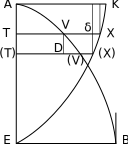
\includegraphics[width=0.28\textwidth]{gesamttex/edit_VIII,3/images/LH_37_05_180_d2.pdf}}%
  \vspace*{0.5em}
  \centerline{{\normalsize\lbrack\textit{Fig.~2}\rbrack}}%
  \label{LH_37_05_180r_Fig.2}%
  \vspace{1.5em}%
%  \newpage%
%
%
\normalsize%
\count\Bfootins=1000
\count\Afootins=1200
\count\Cfootins=1000
\pstart%
%\noindent%
Rem ergo%
\edlabel{LH_37_05_180_m180r6}
%
de integro ordiamur,%
\protect\index{Sachverzeichnis}{res de integro ordita}
et pro accessibus sumamus%
\protect\index{Sachverzeichnis}{accessus ad terminum}
longinquitates a termino%
\protect\index{Sachverzeichnis}{longiquitas a termino}
seu distantias.%
\protect\index{Sachverzeichnis}{distantia a termino}
Ut res melius oculis subjiciatur:%
\protect\index{Sachverzeichnis}{oculus}
sit
%
\edtext{ergo \textit{AE} tempus%
\protect\index{Sachverzeichnis}{tempus restitutionis}%
}{%
\lemma{ergo}\Bfootnote{%
\textit{(1)}~tempus
\textit{(2)}~\textit{AE} tempus%
~\textit{L}}}
%
quo ad terminum pervenitur,%
\protect\index{Sachverzeichnis}{terminus motus}
inde a primo initio libere ad eum accedendi.
\textit{AK} sit longinquitas,%
\protect\index{Sachverzeichnis}{longiquitas a termino}
seu discessus a termino,%
\protect\index{Sachverzeichnis}{distantia a termino}%
\protect\index{Sachverzeichnis}{terminus motus}
seu
%
\edtext{ipsa maxima violentia,%
\protect\index{Sachverzeichnis}{violentia maxima}
post quam}{%
\lemma{ipsa}\Bfootnote{%
\textit{(1)}~tensio maxima, post quam
\textit{(2)}~maxima violentia, post quam%
~\textit{L}}}
%
relinquitur res sibi%
\protect\index{Sachverzeichnis}{res sibi relicta}
ut se restituere possit.%
\protect\index{Sachverzeichnis}{restitutio rei tensae}
In quovis momento temporis%
\protect\index{Sachverzeichnis}{tempus restitutionis}
%
\edtext{ut \textit{T},
sunto}{%
\lemma{ut \textit{T},}\Bfootnote{%
\textit{(1)}~erunt
\textit{(2)}~sunto%
~\textit{L}}}
%
longinquitates adhuc residuae \textit{TX},%
\protect\index{Sachverzeichnis}{longiquitas residua}
donec tandem momento ultimo%
\protect\index{Sachverzeichnis}{momentum restitutionis ultimum}
%
\edtext{\lbrack\textit{E}\rbrack}{% ,
\lemma{\textit{T}}\Bfootnote{%
\textit{L~ändert Hrsg.}}}
%
omnis longinquitas%
\protect\index{Sachverzeichnis}{longiquitas a termino}
a termino expetito%
\protect\index{Sachverzeichnis}{terminus motus}%
\protect\index{Sachverzeichnis}{terminus expetitus}
evanescat.%
\protect\index{Sachverzeichnis}{longiquitas evanescens}
Itaque illic curva \textit{KXE} occurrit axi.%
\protect\index{Sachverzeichnis}{axis}
\edlabel{LH_37_05_180_utpunctumunum-1}%
Porro id quod movetur
in re ad terminum accedente,%
\protect\index{Sachverzeichnis}{res ad terminum accedens}
consideremus ut unum punctum,%
\protect\index{Sachverzeichnis}{punctum unum}
ne scilicet ipsorum diversorum punctorum%
\protect\index{Sachverzeichnis}{conatus puncti}
%
\edtext{conatus sibi mutuo obstantes%
\protect\index{Sachverzeichnis}{conatus sibi obstantes}
calculum turbent;%
\protect\index{Sachverzeichnis}{turbatio calculi}%
\protect\index{Sachverzeichnis}{calculus turbatus}%
}{%
\lemma{conatus}\Bfootnote{%
\textit{(1)}~rem turbent
\textit{(2)}~sibi mutuo obstantes calculum turbent;%
~\textit{L}}}
%
poterit
%
\edtext{autem (opinor) sumi}{%
\lemma{autem}\Bfootnote{%
\textit{(1)}~sumi
\textit{(2)}~(opinor) sumi%
~\textit{L}}}
%
omnium revera existentium centrum gravitatis,%
\protect\index{Sachverzeichnis}{centrum gravitatis}
cujus directio%
\protect\index{Sachverzeichnis}{directio centri gravitatis}
ipsorum inter se conatibus non turbatur,%
\protect\index{Sachverzeichnis}{directio turbata}%
\protect\index{Sachverzeichnis}{conatus puncti}%
\protect\index{Sachverzeichnis}{conatus sibi obstantes}
et
%
\edtext{ideo}{%
\lemma{ideo}\Bfootnote{%
\textit{erg.~L}}}
%
pro totius directione sumi potest.%
\protect\index{Sachverzeichnis}{directio totius}
Neque aliam hic actionem esse suppono,%
\protect\index{Sachverzeichnis}{actio alia}
quam quae oritur ab ipsa solicitatione%
\protect\index{Sachverzeichnis}{actio orta a solicitatione}%
\protect\index{Sachverzeichnis}{solicitatio accedendi ad terminum}
%
\edtext{accedendi.
Praeterea puncti velocitate licebit%
\protect\index{Sachverzeichnis}{velocitas puncti}%
\lbrack,\rbrack\
opinor%
\lbrack,\rbrack\
repraesentare accessionem formalem%
\protect\index{Sachverzeichnis}{accessio formalis}
a locali diversam%
\protect\index{Sachverzeichnis}{accessio localis}
de qua hoc loco proprie agitur,
cui nescio
an semper respondeat ipsa velocitas%
\protect\index{Sachverzeichnis}{velocitas puncti realis}
alicujus puncti realis%
\protect\index{Sachverzeichnis}{punctum reale}
in ipso mobili assignabilis.%
\protect\index{Sachverzeichnis}{mobile}
Talis est accessio a
\lbrack tensione\rbrack%
\protect\index{Sachverzeichnis}{tensio}
ad statum naturalem.%
\protect\index{Sachverzeichnis}{status naturalis}%
}{%
\lemma{accedendi.}\Bfootnote{%
\textit{(1)}~Hujus puncti
\textit{(a)}~solicitatio
\textit{(b)}~velocitas intelligatur non tam localis, quam formalis, ut si mutatio fiat tensionis
\textit{(2)}~Praeterea puncti % velocitate licebit opinor repraesentare 
\lbrack...\rbrack\ accessionem formalem
\textbar~a locali diversam \textit{erg.}~%
\textbar\ de qua % hoc loco proprie 
\lbrack...\rbrack\ agitur, cui
\textit{(a)}~non
\textit{(b)}~nescio an % semper respondeat ipsa velocitas alicujus puncti realis in ipso mobili assignabilis.
\lbrack...\rbrack\ Talis est
\textit{(aa)}~mutatio
\textit{(bb)}~accensi
\textit{(cc)}~accessio a
\textbar~densitate\protect\index{Sachverzeichnis}{densitas} \textit{ändert Hrsg.}~%
\textbar\ 
ad statum naturalem.%
~\textit{L}}}
%
%%%%%%
An ergo licebit
%
\edtext{in tali quoque}{%
\lemma{in}\Bfootnote{%
\textit{(1)}~hoc quoque
\textit{(2)}~tali quoque%
~\textit{L}}}
%
aestimatione%
\protect\index{Sachverzeichnis}{aestimatio}
considerare velocitatem%
\protect\index{Sachverzeichnis}{velocitas acquisita}%
\protect\index{Sachverzeichnis}{velocitas integra}%
\protect\index{Sachverzeichnis}{velocitas accedendi ad terminum}
%
\edtext{acquisitam}{%
\lemma{acquisitam}\Bfootnote{%
\textit{erg.~L}}}
%
integram accedendi % , 
ut aggregatum solicitationum accedendi,%
\protect\index{Sachverzeichnis}{solicitatio accedendi ad terminum}%
\protect\index{Sachverzeichnis}{aggregatum solicitationis}
inde ab initio sumtarum\lbrack?\rbrack\
Ita liceret
si punctum illud reale%
\protect\index{Sachverzeichnis}{punctum reale}
seu centrum gravitatis%
\protect\index{Sachverzeichnis}{centrum gravitatis}
eadem proportione ferretur.
Hanc ergo saltem
%
\lbrack180~v\textsuperscript{o}\rbrack\    %%%%%    Blatt 180v
%
hypothesin%
\protect\index{Sachverzeichnis}{hypothesis}
sumamus.%
\edlabel{LH_37_05_180_utpunctumunum-2}
Puncti ergo
%
\edtext{hujus%
\lbrack,\rbrack\
motu%
\protect\index{Sachverzeichnis}{motus puncti}
suo per omnia accessum formalem%
\protect\index{Sachverzeichnis}{accessus formalis}
repraesentantis%
\lbrack,\rbrack\
velocitas%
\protect\index{Sachverzeichnis}{velocitas puncti}%
}{%
\lemma{hujus}\Bfootnote{%
\textit{(1)}~cujus velocitas repraesent
\textit{(2)}~motu suo % per omnia accessum formalem 
\lbrack...\rbrack\ repraesentantis velocitas%
~\textit{L}}}
%
initio quidem erit nulla,%
\protect\index{Sachverzeichnis}{velocitas nulla}
postea crescens in momento \textit{T}
erit \textit{TV},
et postremo erit maxima%
\protect\index{Sachverzeichnis}{velocitas maxima}
%
\edtext{\textit{EB}.
Unde}{%
\lemma{\textit{EB}.}\Bfootnote{%
\textit{(1)}~Ubi
\textit{(2)}~Unde%
~\textit{L}}}
%
lineam \textit{AVB} describendo,
%
erunt \textit{D(V)} velocitatum
%\edtext{}{%
%\lemma{erunt}\Bfootnote{%
%\textit{(1)}~\textit{D(V)} ve
%\textit{(2)}~\textit{D(V)} velocitatum%
%~\textit{L}}}
%
\edtext{incrementa,%
\protect\index{Sachverzeichnis}{incrementum velocitatis}
seu solicitationes;%
\protect\index{Sachverzeichnis}{solicitatio accedendi ad terminum}
sed hoc}{%
\lemma{incrementa,}\Bfootnote{%
\textit{(1)}~sed hoc
\textit{(2)}~seu solicitationes; sed hoc%
~\textit{L}}}
%
incrementum postremo evanescet in \textit{E},%
\protect\index{Sachverzeichnis}{incrementum evanenscens}
adeoque \textit{EB} erit maxima,
seu recta
%
\edtext{lineam \textit{AVB} tangens in \textit{B}}{%
\lemma{lineam}\Bfootnote{%
\textit{(1)}~in \textit{B} t
\textit{(2)}~\textit{AVB} tangens in \textit{B}%
~\textit{L}}}
%
erit axi \textit{AE} parallela.%
\protect\index{Sachverzeichnis}{axis}
Erunt
%
\edtext{autem $\delta X$ accessiones%
\protect\index{Sachverzeichnis}{accessio ad terminum}
seu incrementa accessuum%
\protect\index{Sachverzeichnis}{incrementum accessus}%
%
\protect\index{Sachverzeichnis}{accessus ad terminum}}{%
\lemma{autem}\Bfootnote{%
\textit{(1)}~in
\textit{(2)}~$\delta X$
\textit{(a)}~elementa
\textit{(b)}~accessiones seu
\textit{(aa)}~elementa
\textit{(bb)}~incrementa accessuum%
~\textit{L}}}
%
vel decrementa%
\protect\index{Sachverzeichnis}{decrementum longinquitatum}
%
\edtext{longinquitatum,%
\protect\index{Sachverzeichnis}{longiquitas a termino}
in ratione composita}{%
\lemma{longinquitatum,}\Bfootnote{%
\textit{(1)}~proportionalia
\textit{(2)}~in ratione composita%
~\textit{L}}}
%
velocitatum \textit{TV}%
\protect\index{Sachverzeichnis}{velocitas accedendi ad terminum}
et intervallorum temporis \textit{T(T)}.%
\protect\index{Sachverzeichnis}{intervallum temporis}%
\protect\index{Sachverzeichnis}{tempus restitutionis}%
\pend%
%\newpage%
%
%
\pstart%
Assumatur jam aliud intervallum%
\protect\index{Sachverzeichnis}{intervallum temporis}
seu alia
%
\edtext{tensio summa \textit{Ak},%
\protect\index{Sachverzeichnis}{tensio summa}
ubi tempus restitutionis \textit{Ar},%
\protect\index{Sachverzeichnis}{tempus restitutionis}%
}{%
{\lemma{tensio summa \textit{Ak}}\Bfootnote{%
\textit{(1)}~initialis
\textit{(2)}~summa \textit{Ak},
\textit{(a)}~sit tempus r
\textit{(b)}~ubi tempus restitutionis \textit{Ar},%
~\textit{L}}}%
{\lemma{\textit{Ak}}\Cfootnote{%
Vgl. das Diagramm \lbrack\textit{Fig.~3}\rbrack\ auf S.~\pageref{LH_37_05_180v_Fig.3}.}}%
}
%
maxima velocitas restituendo assequenda%
\protect\index{Sachverzeichnis}{velocitas restituendo assequenda}%
\protect\index{Sachverzeichnis}{velocitas maxima}
%
\edtext{$r\beta.$
Quaeritur an coincidat}{%
\lemma{$r\beta$}\Bfootnote{\hspace{-0,5mm}%
\textit{(1)}~, atque adeo coincident vi
\textit{(2)}~. Quaeritur an coincidat%
~\textit{L}}}
%
\textit{Ar} ipsi \textit{AE},
et quomodo se habeat $r\beta.$
Est
%
\edtext{autem solicitatio eadem,%
\protect\index{Sachverzeichnis}{solicitatio accedendi ad terminum}
tensione existente eadem;%
\protect\index{Sachverzeichnis}{tensio elastri}
adeoque eadem tensione deposita,%
\protect\index{Sachverzeichnis}{tensio deposita}
velocitas acquiritur eadem.%
\protect\index{Sachverzeichnis}{velocitas acquisita}%
\protect\index{Sachverzeichnis}{velocitas accedendi ad terminum}%
}{%
\lemma{autem}\Bfootnote{%
\textit{(1)}~rem
\textit{(2)}~solicitatio
\textit{(a)}~proportionalis
\textit{(b)}~et
\textit{(c)}~tensioni, adeoque eaedem erunt solicitationes quae ante fiebant
\textit{(d)}~eadem, tensione % existente eade;, adeoque eadem tensione deposita, velocitas 
\lbrack...\rbrack\ acquiritur eadem.%
~\textit{L}}}
%
Ex puncto \textit{k} ducatur parallela
%
\edtext{}{{\xxref{KZeitz113}{KZeitz114}}%
{%
\lemma{ipsi}\Bfootnote{%
\textit{(1)}~\textit{AE},
\textit{(2)}~lineae
\textbar~\textit{EX} \textit{ändert Hrsg.}~%
\textbar\ in \textit{G}.%
~\textit{L}}}}%
\edlabel{KZeitz113}ipsi
\pend
\newpage
\pstart 
\begin{minipage}[t]{0.5\textwidth}
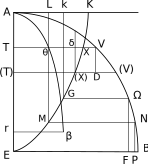
\includegraphics[width=0.76\textwidth]{gesamttex/edit_VIII,3/images/LH_37_05_180_d3.pdf}
\end{minipage}
\hspace{15mm}
\begin{minipage}[t]{0.5\textwidth}
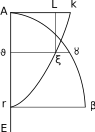
\includegraphics[width=0.5\textwidth]{gesamttex/edit_VIII,3/images/LH_37_05_180_d4.pdf}
\end{minipage}
\\
\\
\hspace*{25mm} [\textit{Fig.~3}]\hspace*{64mm} [\textit{Fig.~4}] \label{LH_37_05_180v_Fig.3}\label{LH_37_05_180v_Fig.4}%
\edtext{}{\lemma{\hspace{1,6mm}\lbrack\textit{Fig.~3}\rbrack\ und \lbrack\textit{Fig.~4}\rbrack}\killnumber\Cfootnote{%
Die Punkte $\theta$ und $\vartheta$ in den zwei Diagrammen entsprechen nicht einander.%
}}%
\pend
\vspace{2.5em}

%%
%%
%%  \newpage% 
%  \vspace*{-0.5em}%	% Diagramm Fig.~3
%  \centerline{\hspace{-70mm}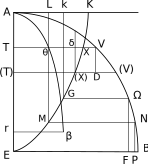
\includegraphics[width=0.38\textwidth]{gesamttex/edit_VIII,3/images/LH_37_05_180_d3.pdf}}% 
%  \vspace*{0.0em}
%  \centerline{\hspace{-70mm}\lbrack\textit{Fig.~3}\rbrack}%
%  \label{LH_37_05_180v_Fig.3}%
%%  \vspace{1.5em}%
%%  \newpage%
%%
%%
%%  \newpage% 
%  \vspace{-15.5em}%	% Diagramm Fig.~4
%  \centerline{\hspace{80mm}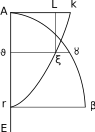
\includegraphics[width=0.25\textwidth]{gesamttex/edit_VIII,3/images/LH_37_05_180_d4.pdf}}% 
%  \vspace*{0.0em}
%  \centerline{\hspace{80mm}\lbrack\textit{Fig.~4}\rbrack}%
%  \label{LH_37_05_180v_Fig.4}%
%%  \vspace{1.5em}%
%%  \newpage%
%%
%
%  \newpage% 
	% Diagramm Fig.~5
  \centerline{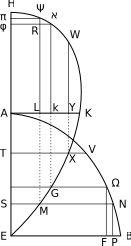
\includegraphics[width=0.30\textwidth]{gesamttex/edit_VIII,3/images/LH_37_05_180_d5.pdf}}%\hspace{30mm}
  \vspace{0.5em}
  \centerline{\lbrack\textit{Fig.~5}\rbrack}%\hspace{30mm}
  \label{LH_37_05_180v_Fig.5}%
    \newpage%
%
\pstart
\noindent lineae \lbrack\textit{EA}\rbrack\
in \textit{G}.%
%
Ex \textit{G} ipsi \textit{AK} ducatur parallela $G\varOmega$\edlabel{KZeitz114}
occurrens ipsi \textit{AV} in $\varOmega,$
%
\edtext{et per $\varOmega$}{%
\lemma{et}\Bfootnote{%
\textit{(1)}~ex $\varOmega$
\textit{(2)}~per $\varOmega$%
~\textit{L}}}
%
agatur parallela ipsi \textit{AE},
occurrens ipsi \textit{EB} in \textit{F}.
Patet
\textit{EF} esse velocitatem jam acquisitam%
\protect\index{Sachverzeichnis}{velocitas acquisita}
tunc
%
\edtext{\lbrack cum\rbrack}{%
\lemma{tum}\Bfootnote{%
\textit{L~ändert Hrsg.}}}
%
tensio in priore casu pervenit ad \textit{Ak},%
\protect\index{Sachverzeichnis}{tensio elastri}
adeoque
%
\edtext{velocitatem hujus quoque tensionis}{%
\lemma{velocitatem}\Bfootnote{%
\textit{(1)}~residuae
\textit{(2)}~hujus quoque tensionis%
~\textit{L}}}
%
depositione%
\protect\index{Sachverzeichnis}{depositio tensionis}
acquirendam esse%
\protect\index{Sachverzeichnis}{velocitas depositione acquirenda}
%
\edtext{\textit{FB},
quae proinde eadem est cum $r\beta$%
}{%
{\lemma{\textit{FB},}\Bfootnote{%
\textit{(1)}~quae eadem est.
\textit{(2)}~quae proinde eadem est cum
\textit{(a)}~\textit{rb}
\textit{(b)}~$r\beta$%
~\textit{L}}}%
{\lemma{\textit{FB} \lbrack...\rbrack\ $r\beta$}\Cfootnote{%
Die Aussage entspricht nicht den Verhältnissen in \lbrack\textit{Fig.~3}\rbrack.}}%
}
%
velocitate acquirenda depositione%
\protect\index{Sachverzeichnis}{velocitas depositione acquirenda}
ejusdem tensionis in%
\protect\index{Sachverzeichnis}{depositio tensionis}
%
\edtext{casu novo,}{%
\lemma{casu}\Bfootnote{%
\textit{(1)}~secundo,
\textit{(2)}~novo,%
~\textit{L}}}
%
si non alia ab initio fuisse intelligatur.
Et generaliter si sit elongatio%
\protect\index{Sachverzeichnis}{elongatio elastri}
%
\edtext{quaecunque
\edtext{$\vartheta\xi$}{%
\lemma{$\vartheta\xi$}\Cfootnote{%
Vgl. das Diagramm \lbrack\textit{Fig.~4}\rbrack\ auf S.~\pageref{LH_37_05_180v_Fig.4}.
Im Folgenden bezieht sich Leibniz aber wieder unmittelbar auf das Diagramm \lbrack\textit{Fig.~3}\rbrack, in dem die Strecke $\vartheta\xi$ nicht vorkommt und der Punkt $\theta$ anders eingezeichnet ist.%
}}
et ducantur ipsis}{%
\lemma{quaecunque}\Bfootnote{%
\textit{(1)}~$T\xi$
\textit{(2)}~$\vartheta\xi$
\textit{(a)}~vel \textit{AL} occurrens ipsi
\textit{(b)}~et ducantur ipsis%
~\textit{L}}}
%
\textit{AE}, \textit{EB} parallelae \textit{LM}, \textit{MN},
occurrentes ipsi \textit{EXK} in \textit{M},
et \textit{NP} parallela \textit{AE},
occurrens ipsi \textit{EB} in \textit{P},
erit \textit{PB} aequalis
$\langle\xi\rangle\!\!\downpropto$
celeritati depositione tensionis
%
\edtext{\lbrack\textit{Lk}\rbrack}{%
\lemma{\textit{LK}}\Bfootnote{%
\textit{L~ändert Hrsg.}}}
%
quaesitae.%
\protect\index{Sachverzeichnis}{celeritas depositione quaesita}%
\protect\index{Sachverzeichnis}{depositio tensionis}
Itaque si
%
\edtext{Tensionibus depositis%
\protect\index{Sachverzeichnis}{tensio deposita}
\edtext{\textit{KY} vel \textit{KL}%
}{%
\lemma{\textit{KY} vel \textit{KL}}\Cfootnote{%
Vgl. das Diagramm \lbrack\textit{Fig.~5}\rbrack\ auf S.~\pageref{LH_37_05_180v_Fig.5}.}}
applicentur velocitates}{%
\lemma{Tensionibus}\Bfootnote{%
\textit{(1)}~applicentur solicitatitiones et
\textit{(2)}~\textit{K}
\textit{(3)}~depositis \textit{KY} vel \textit{KL} applicentur velocitates%
~\textit{L}}}
%
deponendo quaesitae $YW = TV,$%
\protect\index{Sachverzeichnis}{velocitas deponendo quaesita}
vel
%
$L\varPsi = \edtext{SN$ et $AH = EB,$
tunc linea \textit{KW}$\aleph$$\varPsi$\textit{H} repraesentabit}{%
\lemma{\textit{SN}}\Bfootnote{%
\textit{(1)}~repraesentabit itaque linea \textit{KWT}
\textit{(2)}~et $AH = EB,$
\textit{(a)}~utique
\textit{(b)}~tunc linea \textit{KW}$\aleph$$\varPsi$\textit{H} repraesentabit%
~\textit{L}}}
%
velocitates relatas ad tensiones,%
\protect\index{Sachverzeichnis}{velocitas relata ad tensionem}
%
\edtext{et si compleatur rectang. $Ak \aleph \phi,$%
\protect\index{Sachverzeichnis}{rectangulum}%
}{%
\lemma{et}\Bfootnote{%
\textit{(1)}~si sit $\aleph\phi\aleph$
\textit{(2)}~si compleatur rectang. $Ak\aleph\phi,$%
~\textit{L}}}
%
ipsae
%
\edtext{ordinatim}{%
\lemma{ordinatim}\Bfootnote{%
\textit{erg.~L}}}
%
applicatae ad $\aleph\phi$ % ,
a linea $\aleph$$\varPsi$\textit{H}
repraesentabunt velocitates easdem
quae in secundo casu quaeruntur,
ubi maxima tensio%
\protect\index{Sachverzeichnis}{tensio maxima}
non esset % ,
nisi \textit{Ak} vel $\phi\aleph,$
nam velocitas tensionis \textit{kL}
%
\edtext{seu $\aleph R$}{%
\lemma{seu}\Bfootnote{%
\hspace{-0,5mm}$\aleph R$
\textit{erg.~L}}}
%
depositione quaesita%
\protect\index{Sachverzeichnis}{velocitas depositione acquisita}%
\protect\index{Sachverzeichnis}{depositio tensionis}
%
\edtext{foret $\varPsi R$ eadem
quae
\lbrack$\xi\!\!\downpropto$\rbrack%
}{%
\lemma{foret}\Bfootnote{%
\textit{(1)}~\textit{TW} eadem
\textit{(2)}~$\Psi R$ eadem quae
\textit{(a)}~$T\!\!\downpropto$
\textit{(b)}~\textbar~$\vartheta\!\!\downpropto$ \textit{ändert Hrsg.}~\textbar%
~\textit{L}}}
%
in casu secundo.
Sed nunc investigandum tempus%
\protect\index{Sachverzeichnis}{tempus restitutionis}
%
\edlabel{LH_37_05_180_m180v1}%
\textit{Ar}.%
%
\edtext{}{%
{\xxref{LH_37_05_180_m180v1}{LH_37_05_180_m180v2}}%
{\lemma{\textit{Ar}.}\Bfootnote{%
\textit{(1)}~\lbrack/\rbrack\ Sit \textbar\ et \textit{gestr.} \textbar\ tensio \textit{x}, tensio tota
\textit{(a)}~$K + x,$
\textit{(b)}~\textit{K}, tensio deposita
\textit{(2)}~\lbrack/\rbrack\ Sit tensio % \textit{x} residua, tensio tota \textit{K}; tensio 
\lbrack...\rbrack\ deposita $K - x$
\textit{(a)}~solicitatio
\textit{(b)}~velocitas%
~\textit{L}}}}%
%\pend%
%\newpage%
%%
%\pstart%
%%
\edtext{}{%
\lemma{\textit{Nebenrechnung:}}\Afootnote{%
$\displaystyle\frac{dx}{K + x} + \displaystyle\frac{dx}{K - x}
=
\displaystyle\frac{2Kdx}{KK - xx}$%
\newline%
}}%
\pend%
%
\pstart%
Sit tensio \textit{x} residua,%
\protect\index{Sachverzeichnis}{tensio residua}
tensio tota \textit{K},% ;%
\protect\index{Sachverzeichnis}{tensio tota}
tensio deposita $K-x,$%
\protect\index{Sachverzeichnis}{tensio deposita}
velocitas%
\edlabel{LH_37_05_180_m180v2}
%
deponendo quaesita \textit{v},%
\protect\index{Sachverzeichnis}{velocitas deponendo quaesita}
et \textit{dv} incrementum velocitatis%
\protect\index{Sachverzeichnis}{incrementum velocitatis}
%
\edtext{pendet a tensione residua \textit{x}%
\protect\index{Sachverzeichnis}{tensio residua}
seu per eam solam determinatur%
\lbrack;\rbrack\
porro \textit{dx}%
}{%
\lemma{pendet}\Bfootnote{%
\textit{(1)}~ita
\textit{(2)}~a tensione residua \textit{x}
\textit{(a)}~ita ut eadem
\textit{(b)}~seu per eam solam determinatur
\textit{(aa)}~porro tunc \textit{dx\,ddx} e
\textit{(bb)}~posito
\textit{(cc)}~porro
\textit{(aaa)}~\textit{dx}
\textit{(bbbb)}~\textit{dx}%
~\textit{L}}}
%
accessiones ad terminum,%
\protect\index{Sachverzeichnis}{accessio ad terminum}
seu decrementa%
\protect\index{Sachverzeichnis}{decrementum tensionis}
vel depositiones
%
\edtext{tensionum,%
\protect\index{Sachverzeichnis}{depositio tensionis}
sunt ut \textit{v\,dt}}{%
\lemma{tensionum,}\Bfootnote{%
\textit{(1)}~sunt ut
\textit{(a)}~\textit{t}
\textit{(b)}~\textit{x\,dt}
\textit{(2)}~sunt ut \textit{v\,dt}%
~\textit{L}}}
%
adeoque $dx\stackrel{(1)}{=}v\,dt:a,$
posito
%
\edtext{\lbrack\textit{a}\rbrack}{%
\lemma{\textit{b}}\Bfootnote{%
\textit{L~ändert Hrsg.}}}
%
esse certam quandam
%
\edtext{velocitatem \textit{h}%
\protect\index{Sachverzeichnis}{velocitas accedendi ad terminum}
seu%
}{%
\lemma{velocitatem}\Bfootnote{%
\textit{(1)}~maximam \textit{EB}
\textit{(2)}~\textit{h}
\textit{(a)}~\textit{A}
\textit{(b)}~\textit{EB}
\textit{(c)}~porro veloci
\textit{(d)}~si jam
\textit{(e)}~seu%
~\textit{L}}}
%
$t \stackrel{(2)}{=} \displaystyle h \!\!\int\!\!\overline{dx : v}.$
\pend%
%
\pstart%
In secundo casu,%
\protect\index{Sachverzeichnis}{casus}
sit tempus \textit{(t)}%
\protect\index{Sachverzeichnis}{tempus restitutionis}
\edlabel{LH_37_05_180_m180v3}%
et%
%
%
\edtext{}{%
{\xxref{LH_37_05_180_m180v3}{LH_37_05_180_m180v4}}%
{\lemma{et}\Bfootnote{%
\textit{(1)}~\textit{dx}
\textit{(2)}~et
\textit{(3)}~initia
\textit{(4)}~tensio initialis
\textit{(a)}~sit \textit{(K)}
\textit{(b)}~seu tota
\textit{(c)}~seu prima sit \textit{(K)}
\textit{(aa)}~. Et \textit{v} quidem paulo \textlangle an\textrangle\
\textit{(bb)}~, et solicitatio
\textit{(aaa)}~primum est \textit{Y}
\textit{(bbb)}~prima \textit{Y} pendet ex \textit{K},
\textit{(aaaa)}~seu est
\textit{(bbbb)}~seu $d\textit{(v)} = \textit{(\text{\~{K}})},$
\textit{(aaaaa)}~secunda est
\textit{(bbbbb)}~secunda $[2]\, d\textit{(v)},$
\textit{(aaaaa-a)}~pendet a
\textit{(bbbbb-b)}~$K - [1]\, d\textit{(x)},\ [3]\,d\textit{(v)} = \textit{(K)} - [2]\, dx$ seu est $d\textit{(v)} = \textit{(\text{\~{x}})}$
\textit{(5)}~Tensio residua % ...
\lbrack...\rbrack\ ut $dv = \textit{\text{\~{x}}}.$%
~\textit{L}}}%
{\lemma{et \lbrack...\rbrack\ $dv = \textit{\text{\~{x}}}$}\Cfootnote{%
Die eckigen Klammern in Unterstufen der gestr. Variante \textit{(4)} stammen von Leibniz.}}}
%
%
Tensio residua%
\protect\index{Sachverzeichnis}{tensio residua}
seu deponenda \textit{x}%
\protect\index{Sachverzeichnis}{tensio deponenda}
fit
$d\textit{(}v\textit{)} = \textit{(\text{\~{x}})}$
ut
$dv = \textit{\text{\~{x}}}.$%
\edlabel{LH_37_05_180_m180v4}%
%
%
\edlabel{LH_37_05_180_rndbmerk_2-1}%
\edtext{}{%
\lemma{\textit{Am Rand:}}\Afootnote{%
NB NB%
\textsuperscript{\lbrack a\rbrack}
Peccavi in eo
quod posui%
\textsuperscript{\lbrack b\rbrack}
elementare ordinario,%
\protect\index{Sachverzeichnis}{elementare ordinario proportionale}
nempe \textit{dv},
ipsi \textit{\~{x}}
proportionale\lbrack,\rbrack\
cum dicendum sit
$dv:dx=\text{\textit{\~{x}}}$
et ita alia scheda%
\textsuperscript{\lbrack c\rbrack}%
\protect\index{Sachverzeichnis}{scheda}
rem egregie absolvi.%
{\footnotesize%
\newline\vspace{-0.5em}%
\newline%
%
\textsuperscript{\lbrack a\rbrack}~NB NB
\textit{erg.~L}%
\quad%
%
\textsuperscript{\lbrack b\rbrack}~posui
\textit{(1)}~$dv=\text{\textit{\~{x}}}$
\textit{(2)}~elementare ordinario % nempe \textit{dv} ipsi 
\lbrack...\rbrack\ \text{\textit{\~{x}}} proportionale%
~\textit{L}%
\quad%
%
\textsuperscript{\lbrack c\rbrack}~alia scheda:
N.~\ref{RK60301}.%
%\newline%
}}}%
\edlabel{LH_37_05_180_rndbmerk_2-2}
%
Sed quia \textit{x} siginificat rectam,
ideo ut lex homogeneorum servetur,%
\protect\index{Sachverzeichnis}{lex homogeneorum}
quia tensio revera est solicitationi homogenea,%
\protect\index{Sachverzeichnis}{tensio solicitationi homogenea}%
\protect\index{Sachverzeichnis}{solicitatio accedendi ad terminum}
sumatur constans quaedam solicitatio,%
\protect\index{Sachverzeichnis}{solicitatio constans}
qualis
%
\edtext{est gravitatio infinite parva%
\protect\index{Sachverzeichnis}{gravitatio infinite parva}%
}{%
\lemma{est}\Bfootnote{%
\textit{(1)}~gravitatis
\textit{(2)}~gravitatio infinite parva%
~\textit{L}}}
%
$d\beta$
et fiet
$dv = d\beta\, \textit{\text{\~{x}}}.$
\edlabel{LH_37_05_180v_series infinita-1}%
Sit $dv : d\beta = 10 + 11x + 12xx + 13x^3$
%
\edtext{etc.
Porro
cum \textit{x} sit ipsi \textit{dv}
sive $d\beta$ homogenea,
erit \textit{dx} ipsi \textit{ddv} homogenea,
et si $d\beta$ constans,
erit $d\beta\, d\beta = a\,dx.$%
}{%
\lemma{etc.}\Bfootnote{%
\textit{(1)}~Sit autem $dx = d\beta : a,$ talem enim licet supponere ob homogeneitatem tensionis cum gravitate et
\textit{(a)}~incrementum
\textit{(b)}~incrementi ejus cum gravitate infinite parva
\textit{(2)}~Porro cum \textit{x} sit ipsi \textit{dv}
\textbar~sive $d\beta$ \textit{erg.}~%
\textbar\ homogenea, erit \textit{dx} ipsi \textit{ddv} homogenea,
\textit{(a)}~seu ipsi $dd\beta,$ eritque $d\beta$
\textit{(b)}~et si % $d\beta$ constans, erit 
\lbrack...\rbrack\ $d\beta\, d\beta = a\,dx.$%
~\textit{L}}}
%
Quia ergo licet scribere
$dv\,d\beta = d\beta\, d\beta\,\text{\textit{\~{x}}}$
et $dv\,d\beta = a\,dx\,\text{\textit{\~{x}}},$
seu
%
\edtext{omissa \textit{a},
quae prout opus ad legem supplenda,
fiet}{%
\lemma{omissa \textit{a},}\Bfootnote{%
\textit{(1)}~erit
\textit{(2)}~quae prout \lbrack...\rbrack\ supplenda, fiet%
~\textit{L}}}
%
$dv\,d\beta = dx\,\textit{\text{\~{x}}}.$
Sit
$dv = 10 + 11x + 12x^2,$
etc.
et fiet
%
\edtext{}{%
{\xxref{LH_37_05_180_m180v5}{LH_37_05_180_m180v6}}%
{\lemma{utique}\Bfootnote{%
\textit{(1)}~$\displaystyle v\,d\beta = f + 10x + \frac{1}{2} 11xx + \frac{1}{3} 12x^3$ etc.
\textit{(2)}~$\displaystyle v\,d\beta = \protect\begin{array}[t]{r} +\,10K\\-\phantom{10}x\protect\end{array} + \displaystyle \frac{1}{2} 11 \left\{\protect\begin{array}{l}KK\\-\,xx\protect\end{array}\right . $ etc.%
~\textit{L}}}}%
%
\edlabel{LH_37_05_180_m180v5}%
utique
$\displaystyle v\,d\beta =
\underset{\displaystyle-\ \phantom{40}x}{+\,10K}
%\hspace{-1,5mm}
%\begin{array}[t]{r} +\,10K\\
%-\phantom{10}x\end{array}
\displaystyle + \frac{1}{2}11
\left\{\hspace{-1,5mm}%
\underset{\displaystyle-\;xx}{\phantom{-j}\;KK}
%\begin{array}{l}KK\\
%-\,xx\end{array}
\right.$
etc.%
\edlabel{LH_37_05_180_m180v6}
%
ubi pro tota velocitate%
\protect\index{Sachverzeichnis}{velocitas accedendi ad terminum}
%
\edtext{habenda%
\lbrack,\rbrack\
est sumenda
$x = 0,$}{%
\lemma{habenda}\Bfootnote{%
\textit{(1)}~fiet p
\textit{(2)}~et pro
\textit{(3)}~est sumenda \textit{x}
\textit{(a)}~maxima
\textit{(b)}~$=\,0,$%
~\textit{L}}}
%
et fiet
$d\beta\, v = EB\,d\beta = 10K + \overline{1 : 2}\; 11KK + \overline{1 : 3}\; 12K^3$
%
\edlabel{LH_37_05_180_m180v7}%
etc.%
\edlabel{LH_37_05_180v_series infinita-2}%
%
\edtext{}{%
{\xxref{LH_37_05_180_m180v7}{LH_37_05_180_m180v8}}%
{\lemma{etc.}\Bfootnote{%
\textit{(1)}~Hinc cum experimento constet esse \textit{EB} integras velocitates in duplicata%
\protect\index{Sachverzeichnis}{experimentum}
\textit{(2)}~Quod si consideremus,%
~\textit{L}}}}%
%
\pend%
\newpage
%\vspace{1.0em}%
%
\pstart%
\noindent%
\lbrack\textit{Nachfolgend kleingedruckter Text in L gestrichen:}\rbrack\
\pend%
\vspace{0.5em}%
%
\footnotesize%
\pstart%
\noindent%
%
Quod si consideremus%
\edlabel{LH_37_05_180_m180v8}
in valore ipsius \textit{dv}%
\protect\index{Sachverzeichnis}{valor}
per \textit{x} et $d\beta$
seu $a\,dx : d\beta$
non posse aliquid ipsi \textit{K} homogeneum facile occurrere,
seu ipsi \textit{dv},
consequens est
%
\edtext{\lbrack ut\rbrack}{%
\lemma{ut}\Bfootnote{\textit{erg. Hrsg.}}}
%
faciamus \textit{dv} ut
%
\edtext{\textit{x\,dx},
seu \textit{v} ut \textit{xx},
et fiet}{%
\lemma{\textit{x\,dx},}\Bfootnote{%
\textit{(1)}~fiet ergo
\textit{(2)}~seu \textit{v} ut \textit{xx}, et fiet%
~\textit{L}}}
%
$\displaystyle t = -b \!\int\!\!\overline{dx : xx}$
seu $t = b : x$ % , 
(\protect\vphantom)%
quia
% reciproc
crescentibus \textit{t},
descrescunt \textit{x}%
\lbrack\protect\vphantom(),\rbrack\
seu $x = t : dv,$
$t = b : dv.$
Sed in casu
%
\edtext{ultimi \textit{dv} est constans,
cum ejusdem tensi vim patientis%
\protect\index{Sachverzeichnis}{corpus tensum vim patiens}
ultima solicitatio%
\protect\index{Sachverzeichnis}{solicitatio ultima}
semper sit eadem,
seu ultima tensio,%
\protect\index{Sachverzeichnis}{tensio ultima}%
}{%
\lemma{ultimi}\Bfootnote{%
\hspace{-0,5mm}\textit{dv}
\textit{(1)}~$=\,dt$
\textit{(2)}~est constans.
\textit{(a)}~Cum ultima
\textit{(aa)}~resid
\textit{(bb)}~solicitatio semper sit eadem, quaecunque sit prima,
\textit{(b)}~Cum ejusdem % tensi vim 
\lbrack...\rbrack\ patientis ultima
\textit{(aa)}~cons
\textit{(bb)}~solicitatio
\textit{(aaa)}~semper sit eadem seu vis
\textit{(bbb)}~semper sit % eadem, seu 
\lbrack...\rbrack\ ultima tensio,%
~\textit{L}}}
%
a quacunque demum violentia%
\protect\index{Sachverzeichnis}{violentia}
%
\edtext{redierit.
Cum ergo etiam \textit{b} sit constans
et \textit{dv} sit constans,
etiam $b : dv,$
seu \textit{t},
erit constans.
Et si%
}{%
\lemma{redierit.}\Bfootnote{%
\textit{(1)}~Hinc ergo etiam \textit{t} seu $b : dv$
\textit{(2)}~Cum ergo % etiam \textit{b} sit constans et \textit{dv} sit constans, etiam $b : dv,$ seu \textit{t}, 
\lbrack...\rbrack\ erit constans. Et
\textit{(a)}~\textlangle ne\textrangle\
\textit{(b)}~si%
~\textit{L}}}
%
quis objiciat,
etsi \textit{dv} sit ut \textit{x\,dx},
posse \textlangle tamen\textrangle\ esse \textit{v}
\textlangle non\textrangle\ ut \textit{xx},
sed ut
%
\edtext{$xx + cc;$
videndum quid respondeamus.%
}{%
\lemma{$xx + cc;$}\Bfootnote{%
\hspace{-0,5mm}
\textit{(1)}~resp. Hoc posito non simul rescunt\lbrack\textit{!}\rbrack\ \textit{v} et \textit{x}
\textit{(2)}~videndum quid respondeamus.%
~\textit{L}}}
%
%\textit{(a)}~
%\textit{(b)}~
%\textit{(aaaaa-aaaaa)}~
%\textit{(bbbbb-bbbbb)}~
%
\textlangle Ut\textrangle\ quidem sit \textit{dv} ut \textit{x\,dx},
utique patet.
Sed revera non potest esse \textit{v} ut \textit{xx},
quia \textit{x} decrescunt,
%
\edtext{\lbrack crescentibus\rbrack}{%
\lemma{rescentibus}\Bfootnote{%
\textit{L~ändert Hrsg.}}}
%
\textit{v}.
Ergo fieret \textit{v} ut $KK - xx,$
ita enim initio \textit{v} nulla,
in fine autem ut \textit{KK},
ergo
%
$\displaystyle t =
\edtext{-\,\,b \!\int\!\! \overline{dx :,\, \overline{KK - xx}}.$
Sed nihilominus obtinetur idem.%
}{%
\lemma{$\displaystyle-\,b \!\int\!\! \overline{dx :,\, \overline{KK - xx}}.$}\Bfootnote{%
\textit{(1)}~Unde \textlangle in usu\textrangle\
\textit{(2)}~Sed nihilominus obtinetur idem.%
~\textit{L}}}
%
Et quod pulcherrimum est,%
\protect\index{Sachverzeichnis}{pulcherrimum}
video tandem
quaecunque sit relatio inter \textit{dv} et \textit{x},%
\protect\index{Sachverzeichnis}{relatio}
haberi quaesitum.%
\protect\index{Sachverzeichnis}{quaesitum}
Nempe fiet
$\displaystyle t = -\,b \!\int\!\! \overline{dx \textit{\text{\~{x}}}}$,
ubi nulla alia indeterminata calculum ingreditur quam \textit{x}.%
\protect\index{Sachverzeichnis}{indeterminata calculum ingrediens}%
\protect\index{Sachverzeichnis}{calculus}
Sed \textit{x} determinatur similiter per \textit{dv}
quia $\displaystyle dv = \textit{\text{\~{x}}}$,
ita ut nulla alia indeterminata calculum ingrediatur.%
\protect\index{Sachverzeichnis}{indeterminata calculum ingrediens}%
\protect\index{Sachverzeichnis}{calculus}
Ergo \textit{t} determinatur per solam \textit{dv}
%
\edtext{sine alia indeterminata.%
\protect\index{Sachverzeichnis}{indeterminata calculum ingrediens}
In casu autem ultimi%
\protect\index{Sachverzeichnis}{casus ultimi}
non alia homogenea calculum ingreditur%
\protect\index{Sachverzeichnis}{homogenea calculum ingrediens}%
\protect\index{Sachverzeichnis}{calculus}%
}{%
\lemma{sine alia indeterminata.}\Bfootnote{%
\textit{(1)}~Imo non esse aliam homog.
\textit{(2)}~In casu % autem ultimi non alia homogenea 
\lbrack...\rbrack\ calculum ingreditur%
~\textit{L}}}
%
quam \textit{K},
quia et \textit{x} est \textit{K}.
Sed \textit{x} determinatur similiter per \textit{dv},
quia $dv = \textit{\text{\~{x}}},$
ita ut nulla alia indeterminata calculum ingrediatur.%
\protect\index{Sachverzeichnis}{indeterminata calculum ingrediens}%
\protect\index{Sachverzeichnis}{calculus}
Ergo \textit{t} necessario est $b : K.$
Sed hinc non prodit tempus idem.%
\protect\index{Sachverzeichnis}{tempus restitutionis}%
\protect\index{Sachverzeichnis}{isochronismus restitutionis}
%
\pend%
\vspace{1.0em}%
%\newpage%
%
\normalsize%
\pstart%
\noindent%
Consideramus ergo \textit{v}
ut homogeneum ipsi \textit{x},
reductis omnibus ad lineas,%
\protect\index{Sachverzeichnis}{reductio ad lineas}
quod et ostendit aeq.~2.
Jam veniamus ad
$\displaystyle t = h \!\int\!\!\overline{dx:v}.$
Hinc \textit{t} est ad \textit{h},
ut
%
\edtext{numerus quidam indeterminatus%
\protect\index{Sachverzeichnis}{numerus indeterminatus}%
}{%
\lemma{\textit{Am Rand:}}\Afootnote{%
Non datur Numerus indeterminatus%
\textsuperscript{\lbrack a\rbrack}
ordinarius%
\protect\index{Sachverzeichnis}{numerus ordinarius}
quem una solum homogenea ingrediatur,
sed datur transcendens,%
\protect\index{Sachverzeichnis}{numerus transcendens}
ut $\displaystyle\!\!\int\!\!\frac{dx}{x}.$
%
{\footnotesize%
\newline\vspace{-0.5em}%
\newline%
\textsuperscript{\lbrack a\rbrack}~indeterminatus
\textit{(1)}~qui non sit homogeneus Logarithmo%
\protect\index{Sachverzeichnis}{logarithmus}
\textit{(2)}~ordinarius quem % una solum 
\lbrack...\rbrack\ homogenea ingrediatur,%
~\textit{L}%
\newline%
%
}}}
%
(\protect\vphantom)%
$\displaystyle\!\!\int\!\! \overline{dx : v}$%
\protect\vphantom()
ad unitatem.%
\protect\index{Sachverzeichnis}{unitas}
Quia autem \textit{v} datur in casu ultimi,%
\protect\index{Sachverzeichnis}{casus ultimi}
seu \textit{EB},
ex sola \textit{K},
nec alia homogenea intervenire potest,%
\protect\index{Sachverzeichnis}{homogenea calculum ingrediens}
hinc necesse est
in casu ultimi%
\protect\index{Sachverzeichnis}{casus ultimi}
$\displaystyle\!\int\!\!\overline{dx : v}$
vel esse numerum aliquem absolutum,%
\protect\index{Sachverzeichnis}{numerus absolutus}
v.\,g.
%
\edtext{rat. diam. ad circumf.,%
\protect\index{Sachverzeichnis}{ratio diametri ad circumferentiam}%
\protect\index{Sachverzeichnis}{circumferentia}%
\protect\index{Sachverzeichnis}{diameter}%
}{%
\lemma{rat. diam. ad circumf.}\Cfootnote{%
\textit{rationem diametri ad circumferentiam}}}
%
aut tale quid;
vel esse aliquid logarithmo%
\protect\index{Sachverzeichnis}{logarithmus}
ipsius \textit{K} proportionale.
%
\edtext{%
\edlabel{LH_37_05_180_rndbmerk_3-1}%
Et quidem
si summabilis est
$\displaystyle\!\int\!\!\overline{dv : x},$
necesse est,
numerum oriri constantem,%
\protect\index{Sachverzeichnis}{numerus constans}
seu tempus esse semper idem.%
\edlabel{LH_37_05_180_rndbmerk_3-2}%%
\protect\index{Sachverzeichnis}{tempus restitutionis}%
\protect\index{Sachverzeichnis}{isochronismus restitutionis}%
}{%
\lemma{\textit{Am Rand:}}\Afootnote{%
NB NB
\newline%
}}
%
Exempli causa%
\protect\index{Sachverzeichnis}{exemplum}
sint solicitationes tensionibus proportionales%
\protect\index{Sachverzeichnis}{solicitatio tensioni proportionalis}%
\protect\index{Sachverzeichnis}{solicitatio accedendi ad terminum}%
\protect\index{Sachverzeichnis}{tensio solicitationi proportionalis}
seu \textit{dv} ut \textit{x},
sive \textit{v} ut $KK - xx : K,$
%
\edtext{et \textit{t} ut
$\displaystyle \!\int\!\! dx : v,$}{%
\lemma{et}\Bfootnote{%
\textit{(1)}~$\displaystyle t = h \!\int\!\! dx$
\textit{(2)}~\textit{t} ut $\displaystyle \!\int\!\! dx : v,$%
~\textit{L}}}
%
ut
$K \displaystyle \!\int\!\!\overline{dx : KK - xx},$
seu ut
$\displaystyle \frac{1}{2} \log \overline{K + x} + \displaystyle \frac{1}{2} \log \overline{K - x}.$
Id est
(\protect\vphantom)%
cum $x = 0$%
\protect\vphantom()
%
\edtext{ut $\log K.$
Sed si esset \textit{v}
ut $K^3 : xx,$%
}{%
\lemma{ut}\Bfootnote{%
\hspace{-0,5mm}$\log K.$
\textit{(1)}~Sed si
\textit{(a)}~\textit{v} esset ut
\textit{(b)}~$KK : KK - xx$ ut
\textit{(c)}~\textit{dv} esset ut
\textit{(aa)}~$K \surd x$ seu \textit{v} ut \textit{x}
\textit{(bb)}~$K - v$
\textit{(cc)}~$v - K$
\textit{(dd)}~$K + x$
\textit{(2)}~Sed si esset \textit{v} ut $K^3 : xx,$%
~\textit{L}}}
%
foret
$\displaystyle \!\int\!\!\overline{dx : v} =
%
\edtext{K^3\! : 3x^3\!$
et si esset}{%
\lemma{$K^3\! : 3x^3\!$}\Bfootnote{%
\textit{(1)}~et cum
\textit{(2)}~et si esset%
~\textit{L}}}
%
$x = K$
foret
$=\, 3.$
\pend%
%
\pstart%
Sed talia hic locum non habent.
%
Nempe
\edtext{$d\,\overline{YW}$
(\protect\vphantom)%
\textit{dv}%
\protect\vphantom() pendet%
}{%
\lemma{$d\overline{YW}$}\Bfootnote{%
\textit{(1)}~pendet
\textit{(2)}~(\protect\vphantom)\textit{dv}\protect\vphantom() pendet%
~\textit{L}}}
%
ab \textit{AY}.
%
\edtext{%
\edlabel{LH_37_05_180_rndbmerk_4-1}%
Hinc \textit{YW} cum crescat
decrescente \textit{AY},
non potest esse ipsi proportionale,
sed formulae ex \textit{AV} et
%
\edtext{\textit{AK},
et quidem ex formula%
\protect\index{Sachverzeichnis}{formula}
eodem modo se habente%
}{%
\lemma{\textit{AK}}\Bfootnote{%
\textit{(1)}~. Ergo et
\textit{(2)}~, et quidem
\textit{(a)}~utcunque
\textit{(b)}~ex formula
\textit{(c)}~ex formula%
~\textit{L}}}
%
ad \textit{AY} et \textit{AK},
%
ducta in $AK-AY,$%
\edlabel{LH_37_05_180_rndbmerk_4-2}%
}{%
\lemma{\textit{Am Rand:}}\Afootnote{%
NB NB%
\newline%
}}
%
id enim in talibus necessarium,
ut patet ex expressione%
\protect\index{Sachverzeichnis}{expressio per seriem infinitam}
per seriem infinitam%
\protect\index{Sachverzeichnis}{series infinita}
%
\edtext{paulo ante}{%
\lemma{paulo ante}\Cfootnote{%
S.~\refpassage{LH_37_05_180v_series infinita-1}{LH_37_05_180v_series infinita-2}.%
}}
%
\edtext{posita.
Sed talis formula}{%
\lemma{posita.}\Bfootnote{%
\textit{(1)}~Et quidem
\textit{(2)}~Sed talis
\textit{(a)}~sen
\textit{(b)}~formula%
~\textit{L}}}
%
\textit{dx}
%
\edtext{\lbrack dividendi\rbrack}{%
\lemma{dividentis}\Bfootnote{%
\textit{L~ändert Hrsg.}}}
%
vix dabitur
qu\textlangle adra\textrangle tura.%
\protect\index{Sachverzeichnis}{quadratura}
Sane si \textit{v} esset reciproca ipsi \textit{x},
foret \textit{dv} reciproce ipsi \textit{dx},
quod \pgrk{>'atopon}%
\protect\index{Sachverzeichnis}{atopon@\pgrk{>'atopon}}
cum sit tanto major.
\edlabel{LH_37_05_180v_nonassequi-1}%
Hinc tali methodo%
\protect\index{Sachverzeichnis}{methodus}
non possum isochronismum%
\protect\index{Sachverzeichnis}{isochronismus restitutionis}
%
\edlabel{LH_37_05_180v_dmnf-1}
assequi.%
\edlabel{LH_37_05_180v_nonassequi-2}%
%
\edtext{}{%
{\xxref{LH_37_05_180v_dmnf-1}{LH_37_05_180v_dmnf-2}}%
{\lemma{assequi.}\Bfootnote{%
\textit{(1)}~\lbrack/\rbrack\ Quid si fiat
\textit{(a)}~$v = Kx : ,\, K + 2K + 3K$ fiet \textit{dv}
\textit{(b) }$v = Kx ,\, K - x ,\, : K + x$ fiet $dv \,=$
\textit{(2)}~\lbrack/\rbrack\ Quaerendus est valor ipsius \textit{v}
\textit{(a)}~talis, ut compos
\textit{(b)}~, qui formetur % ... 
\lbrack...\rbrack\ habebitur et \textit{dv},%
~\textit{L}}}}%
%
\edlabel{LH_37_05_180_rndbmerk_5-1}%
\edtext{%
%\label{LH_37_05_180v_marg_srh}%
}{%
\lemma{\textit{Am Rand:}}\Afootnote{%
NB:
Haec ad doctrinam de relationibus in genere.%
\protect\index{Sachverzeichnis}{doctrina de relationibus}%
\protect\index{Sachverzeichnis}{relatio in genere}%
}}%
\edlabel{LH_37_05_180_rndbmerk_5-2}%
%
\pend%
%
\pstart%
Quaerendus est valor ipsius \textit{v},%
\protect\index{Sachverzeichnis}{valor}
qui formetur % , 
multiplicando formulam%
\protect\index{Sachverzeichnis}{formula}
ex \textit{K} et \textit{x}
eodem modo formatam per $K - x,$
ita ut $dx : v$ sit summabilis ordinarie.
Et tunc habebitur et \textit{dv},%
\edlabel{LH_37_05_180v_dmnf-2}
seu lex%
\protect\index{Sachverzeichnis}{lex de actione tensionis}
qua possit agere tensio \textit{x},%
\protect\index{Sachverzeichnis}{tensio elastri}
sive solicitatio.%
\protect\index{Sachverzeichnis}{solicitatio accedendi ad terminum}%
\pend%
 \count\Bfootins=1200
\count\Afootins=1200
\count\Cfootins=1200
%
%
%
% % % %    Ende des Textes auf Bl. 180v